\chapter{Transport domain analysis}

In this chapter, we will analyze two variants of the Transport domain: sequential and temporal. To do this, we will describe the datasets
used for devising experiments, and discuss the properties of Transport
that will help us in developing better quality planners.

\section{Problem complexity}

When domain-independent planners solve a sequential Transport problem,
they face a harder task than planners that have access to domain knowledge ahead of time.
For domain-independent planners, deciding whether a plan of a given length exists
(the \textsc{Plan-Length} decision problem) is
an NEXPTIME-complete task
and deciding if a plan exists at all (the \textsc{Plan-Existence} decision problem)
an EXPSPACE-complete task \citep[Table~3.2]{Ghallab2004}.

That does not mean domain knowledge makes Transport easy, as is evident from
the very thorough analysis by \citet{Helmert2001, Helmert2001a}.
We will categorize our problems using Helmert's notation to
be able to interpret their results to our domain.
Helmert's \textsc{Transport} task is a 9-tuple $(V, E, M, P, fuel_0, l_0, l_G, cap, road),$
where:
\begin{itemize}
\item $(V, E)$ is the road graph;
\item $M$ is a finite set of vehicles (mobiles);
\item $P$ is a finite set of packages (portables);
\item $fuel_0 : V \to \N$ is the fuel function;
\item $l_0: (M \cup P) \to V$ is the initial location function;
\item $l_G: P \to V$ is the goal location function;
\item $cap: M \to \N$ is the capacity function; and
\item $road: M \to 2^E$ is the movement constraints function.
\end{itemize}
$V$, $M$, and $P$ are pairwise disjoint.
No Transport domain variants assume movement constraints, therefore, $road$ is a constant
function $road(m) = E$.
Fuel constraints are modeled differently than in Transport (constraints per location versus per vehicle). \TODO{explain why it doesn't matter complexity-wise}

A simplified notation is also introduced by \citet{Helmert2001a} for special cases of \textsc{Transport} tasks.
For $i,j \in \{1, \infty, *\}, k \in \{1, +, *\}$ a $\textsc{Transport}_{i,j,k}$ task is defined as a
general \textsc{Transport} task (defined above) that satisfies:
\begin{itemize}
\item if $i=1$, then $\forall m \in M : cap(m) = 1$ (vehicles can only carry one package);
\item if $i=\infty$, then $\forall m \in M : cap(m) = |P|$ (vehicles have unlimited capacity);
\item if $j=1$, then $\forall v \in V : fuel_0(v) = 1$ (one fuel unit per location);
\item if $j=\infty$, then $\forall v \in V : fuel_0(v) = \infty$ (unlimited fuel per location);
\item if $k=+$, then $\forall m \in M : road(m) = E$ (no movement restrictions); and
\item if $k=1$, then $M = \{m\} \And road(m) = E$ (single vehicle, no restrictions).
\end{itemize}
The $*$ value for $i$, $j$ or $k$ signifies no restriction on that property.
Note that
\textsc{Transport} refers to the notation of \citet{Helmert2001a} of a general transportation
task, while Transport refers to our studied domain.

Using this notation, the sequential Transport domain could be thought of as a $\textsc{Transport}_{c,\infty,+}$ task, where $c \in \N$
(equivalent to $\textsc{Transport}_{1,\infty,+}$).
Similarly, the temporal variant represents a $\textsc{Transport}_{c,f,+}$ task, for $c, f \in \N$
(equivalent to $\textsc{Transport}_{1,1,+}$).

For sequential and temporal Transport without fuel, the \textsc{Plan-Existence} problem
reduces to verifying reachability of each package by at least one vehicle
and the reachability of target locations from the starting locations of all packages,
which we can do in polynomial time, as noted by \citet[Theorem 8]{Helmert2001}.
With fuel, there is no straightforward way of determining
if a plan exists and this problem is NP-complete, which is proven in \citet[Theorem 9 and 10]{Helmert2001}.

Similarly, the \textsc{Plan-Length} problem is NP-complete for all mentioned variants of Transport
\citep[Section~3.6]{Helmert2001a}.
The fact that all the mentioned proofs work for temporal variants is explained in \citet[Section~3.5]{Helmert2001a}.
All of these results make clear that looking for an explicit planning algorithm is infeasible,
despite the knowledge we acquire by only focusing on one planning domain.














\section{Domain information}\label{domain-info}

There are several interesting properties and invariants that hold in both sequential and temporal Transport and might prove useful for designing planners:
\begin{enumerate}
\item \textbf{Do not pick up delivered packages}: The simplest and trivially correct decision is to never touch packages that are already at their destinations --- there is nothing
we can do using those packages that would result in a plan with a lower total cost.

\item \textbf{Drop when at the destination}: Likewise, it is
always correct for a vehicle containing a package with a destination equal
to the vehicle's location to do a \drop{} action immediately.

\item \textbf{Do not drop and pick up}: It never makes sense to plan a \drop{} and \pickup{}
action of
the same package by the same vehicle in succession. We will only get to the same state
by using a longer plan. This rule also applies if an action of a different vehicle
gets between the two successive actions --- even if it does an action with the
dropped package.
It is important to note that this is a symmetric property: picking up and dropping
equally results in a worse plan.
\begin{enumerate}
\item \textbf{Do not drop package where we picked it up}: A generalization
of the previous rule is that vehicles should never drop a package
at the location they last picked it up, independent of the actions they took
between the relevant \pickup{} and \drop{}. This rule is also symmetric.

\item \textbf{Never drop after picking up at a vertex}:
While the order of successive \pickup{} and \drop{} actions does not
influence the optimality of a plan, it makes the search space smaller and the implementation of these rules simpler,
without sacrificing admissibility. \textit{Admissibility} is
a property of search strategies in general and can be defined as finding
(one of) the optimal solutions (first), when there are generally several solutions
of possibly different qualities \citep[Section~3.5]{Russell1995}.
\end{enumerate}

\item \textbf{Do not drive suboptimally}: If a vehicle does a series of
\drive{} actions from location $A$ to $B$ without ``touching'' packages at any of the locations it visits,
it has to follow the shortest possible path from $A$ to $B$. If it does not,
the induced plan can be made less costly or shorter by swapping the actual \drive{} actions
for precalculated optimal \drive{} actions along the shortest path.
Do note, that it is not important for the application of this rule whether actions are in direct succession (in a sequential plan) or not.
\begin{enumerate}
\item \textbf{Do not drive in cycles}: A special but important case of the previous rule is that vehicles should not drive in cycles
\end{enumerate}

\item \textbf{Do not forward packages using other vehicles}:
Let $p$ be a package of size $|p|$ located at $A$.
Let $v$ be a vehicle which drove through location $A$ to location $B \neq A$
and picked up $p$ at $B$,
without having less than $|p|$ free space in any intermediate state between leaving $A$ and picking up $p$.
If this sequence of events occurs, the plan is suboptimal in a sequential setting, because
$v$ could have picked up $p$ when driving through $A$, and the total plan cost
would have gone down by at least 2. The reason is that a different vehicle had to pick up, drive, and drop package $p$ at $B$.
While we cannot say if the \drive{} action itself
was redundant, the \pickup{} and \drop{} actions definitely were, thereby saving
2 on the total cost. 

In a temporal domain without fuel, assuming that vehicles only drive along the shortest routes,
the plan does not necessarily have to be suboptimal, but it
is of equal length or longer: due to concurrent actions, the vehicles could have driven simultaneously.
In a few cases, the other vehicle could have dropped $p$ at $B$ before $v$ wants to pick it up,
which means that the total makespan of the partial plan did not become longer, but stayed the same.
The plan could not have become shorter, because $v$ does not have any time in this scenario when it is available to do another action.

In a temporal domain with fuel, it is not safe to say whether
such a scenario hurts the plan duration. If there is a petrol station at $B$
and $v$ wants to refuel there, the other vehicle could have enabled the parallelization 
of the \refuel{} and \pickup{} actions, therefore shaving off 1 time unit in total.
However, if there is no petrol
station at $B$, this situation reduces to the no-fuel variant. Given the relative rarity of petrol stations, this will reduce the search space somewhat.
\end{enumerate}
Several other insights can only be applied in the sequential variant of Transport:
\begin{enumerate}
\item \textbf{Drop from an active vehicle only}: Without loss of generality,
we can prune all plans where a \drop{} action of a vehicle happens
right after an action of a different vehicle. It is trivial to see that if we had a plan where
a \drop{} action
occurs after an action of a different vehicle, we can swap that action with the \drop{} action without (a) changing the total plan cost (b) changing the validity of the plan.

Doing this repeatedly will yield an equivalent plan, in which the \drop{} action
occurs right after a different action of the same vehicle and the plan is of the same total cost and validity as the original plan. Repeating this process for each \drop{} action will yield an equivalent plan to the original plan, thus we see that a not-pruned plan of the same length and validity to the same final state exists.
\end{enumerate}
Finally, these are the useful properties that only meaningfully apply to the temporal variant:
\begin{enumerate}
\item \textbf{Refueling and dropping/picking up can occur at the same time}: 
A plan in which a vehicle starts to pick up a package at the same location it refueled at is suboptimal, if there was a time point during the \refuel{} action
when the vehicle was not dropping or picking up packages and the package was already
co-located with the vehicle at that time.

\item \textbf{No fuel left means refueling or ignoring the vehicle}:
If a vehicle is stuck with no fuel left, or with less fuel than is required for
any valid \drive{} action,
the correct thing to do is to either refuel or drop all packages and ignore the vehicle in further planning. Unfortunately,
we cannot say anything about the (non-)optimality of a plan where this occurs.
\end{enumerate}
















\section{Datasets \& problem instances}\label{datasets}

For evaluation and comparison with other planners, we have acquired several problem datasets from previous runs of the IPC.
Table~\ref{tab:ipc-datasets} provides an overview of the individual datasets, their associated IPC competition, the track at the competition and the domain variant the problems are modeled in.

\begin{table}[tb]
\centering
\begin{tabular}{c||ccc}
\textbf{Dataset} & \textbf{Competition} & \textbf{IPC Track} & \textbf{Formulation} \\ 
\midrule
\midrule
netben-opt-6 & IPC-6 & \href{http://icaps-conference.org/ipc2008/deterministic/NetBenefitOptimization.html}{Net-benefit: optimization} & Numeric \\ 
seq-opt-6 & IPC-6 & \href{http://icaps-conference.org/ipc2008/deterministic/SequentialOptimization.html}{Sequential: optimization} & STRIPS \\ 
seq-sat-6 & IPC-6 & \href{http://icaps-conference.org/ipc2008/deterministic/SequentialSatisficing.html}{Sequential: satisficing} & STRIPS \\ 
tempo-sat-6 & IPC-6 & \href{http://icaps-conference.org/ipc2008/deterministic/TemporalSatisficing.html}{Temporal: satisficing} & Temporal \\ 
\midrule
seq-mco-7 & IPC-7 & \href{http://www.plg.inf.uc3m.es/ipc2011-deterministic/SequentialMulticore.html}{Sequential: multi-core} & \multirow{3}{*}{STRIPS} \\ 
seq-opt-7 & IPC-7 & \href{http://www.plg.inf.uc3m.es/ipc2011-deterministic/SequentialOptimization.html}{Sequential: optimization} &  \\ 
seq-sat-7 & IPC-7 & \href{http://www.plg.inf.uc3m.es/ipc2011-deterministic/SequentialSatisficing.html}{Sequential: satisficing} &  \\ 
\midrule
seq-agl-8 & IPC-8 & \href{https://helios.hud.ac.uk/scommv/IPC-14/seqagi.html}{Sequential: agile} & \multirow{4}{*}{STRIPS} \\ 
seq-mco-8 & IPC-8 & \href{https://helios.hud.ac.uk/scommv/IPC-14/seqmulti.html}{Sequential: multi-core} &  \\ 
seq-opt-8 & IPC-8 & \href{https://helios.hud.ac.uk/scommv/IPC-14/seqopt.html}{Sequential: optimization} &  \\ 
seq-sat-8 & IPC-8 & \href{https://helios.hud.ac.uk/scommv/IPC-14/seqsat.html}{Sequential: satisficing} &  \\ 
\end{tabular}
\caption[Transport datasets from the 2008, 2011, and 2014 IPCs.]{Transport datasets from the 2008, 2011, and 2014 IPCs. All formulations assume capacitated vehicles, numeric and temporal formulations also contain fuel demands and capacities. The temporal formulation additionally adds concurrent actions and a notion of time. More information can be found in Section~\ref{domain-desc}.}
\label{tab:ipc-datasets}
\end{table}

Short descriptions of the various tracks and subtracks can be found in the rule pages of IPC-6,\puncfootnote{\url{http://icaps-conference.org/ipc2008/deterministic/CompetitionRules.html}}
IPC-7,\puncfootnote{\url{http://www.plg.inf.uc3m.es/ipc2011-deterministic/CompetitionRules.html}}
and the rule pages of IPC-8.\puncfootnote{\url{https://helios.hud.ac.uk/scommv/IPC-14/rules.html}}
We have decided to split our further research based on the tracks at IPC: we will focus on constructing
Transport-specific planners for the seq-sat-6, seq-sat-7, seq-sat-8, and tempo-sat-6 datasets,
corresponding to the sequential and temporal variants of Transport.

The datasets labeled seq-opt correspond to sequential optimality planning tracks,
where only optimal plans for problems are accepted as correct.
Datasets labeled seq-mco are used in multi-core satisficing tracks (multi-threaded planners)
and seq-agl are used in agile tracks (minimize the CPU time required to find a satisficing plan).
The netben-opt-6 dataset contains Net Benefit problems, where the aim
is to compensate between achieving \textit{soft goals} and minimizing the total cost.
Soft goals are goals that do not necessarily have to be satisfied in a goal state,
but it is usually better for the total score if they are.
Each problem usually specifies a metric used for calculation of the score.
We will not focus on 
these problems in this work.

In addition to the domain definition, we need to take a look at the individual problems to fully utilize our knowledge advantage.
Both the seq-sat-6 and tempo-sat-6 contain 30 problems, while seq-sat-7 and seq-sat-8 only contain 20 problems. Table~\ref{tab:dataset-dimensions} shows the
dimensions of each problem instance for each mentioned dataset.

While the planners (including our domain-specific ones) do not know this,
each problem was constructed with a scenario in mind. Locations in problems are not just
placed randomly, but usually belong to cities. Inside a city, the road network
tends to be dense and road lengths small, while roads connecting cities
are rare and usually significantly longer.


\begin{figure}[tb]
\begin{center}
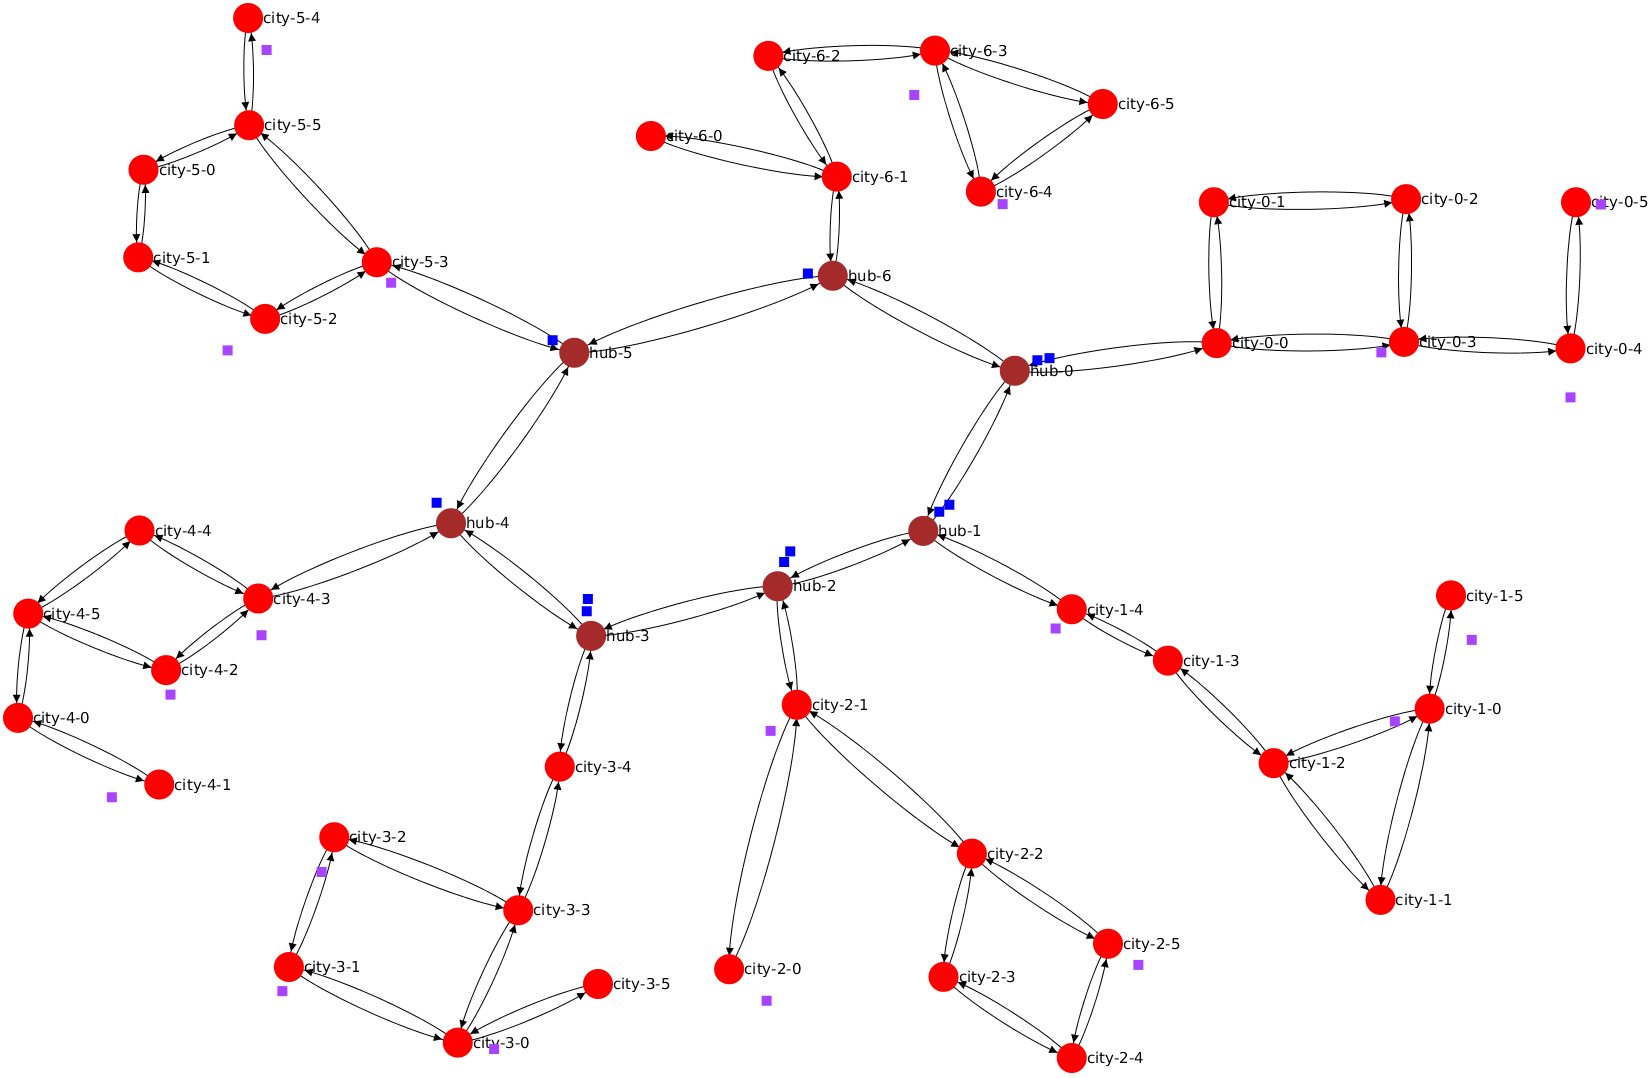
\includegraphics[width=1.0\textwidth]{../img/ipc08_tempo-sat_p30_land}
\end{center}
\caption[Visualization of the \texttt{p30} problem of temporal Transport from IPC 2008.]{Road graph visualization of the \texttt{p30} problem of the tempo-sat track of IPC 2008. Red dots represent locations (graph nodes), roads (graph edges) are represented by black arrows, vehicles are plotted as blue squares, and packages as purple squares. Darker red dots represent locations with petrol stations. In this specific problems, the circle of nodes in the center represents a series of truck hubs and each of the attached subgraphs are individual cities.}
\label{fig:ipc08_tempo-sat_p30}
\end{figure}

\begin{table}[p]
\scriptsize
\centering
\begin{subtable}[t]{0.42\textwidth}
\csvreader[tabular=r||rrrrrl,
    table head=\textbf{\#} & \rot{\textbf{Vehicles}} & \rot{\textbf{Packages}} & \rot{\textbf{Cities}} & \rot{\textbf{Locations}} & \rot{\textbf{Roads}} & \rot{\textbf{States}}\\\midrule\midrule,
    late after line=\mbox{}]
%    table foot=\\\bottomrule]%
{../data/seq-sat-6.csv}{Problem=\problem,Vehicles=\vehicles,Packages=\packages,Cities=\cities,Locations=\locations,%
Roads=\roads,Stateslat=\stateslat}%
{\problem & \vehicles & \packages & \cities & \locations & \roads & \stateslat}%
\caption{Problem dimensions of seq-sat-6.}
\label{tab:seq-sat-6-dims}
\end{subtable}
\quad
\begin{subtable}[t]{0.54\textwidth}
\csvreader[tabular=r||rrrrrrl,
    table head=\textbf{\#} & \rot{\textbf{Vehicles}} & \rot{\textbf{Packages}} & \rot{\textbf{Cities}} & \rot{\textbf{Locations}} & \rot{\textbf{Roads}} & \rot{\textbf{Petrol}} & \rot{\textbf{States}}\\\midrule\midrule,
    late after line=\mbox{}]
%    table foot=\\\bottomrule]%
{../data/tempo-sat-6.csv}{Problem=\problem,Vehicles=\vehicles,Packages=\packages,Cities=\cities,Locations=\locations,%
Roads=\roads,Petrol=\petrol,Stateslat=\stateslat}%
{\problem & \vehicles & \packages & \cities & \locations & \roads & \petrol & \stateslat}%
\caption{Problem dimensions of tempo-sat-6.}
\label{tab:tempo-sat-6-dims}
\end{subtable} 

\vspace{0.5cm}
\begin{subtable}[t]{0.42\textwidth}
\csvreader[tabular=r||rrrrrl,
    table head=\textbf{\#} & \rot{\textbf{Vehicles}} & \rot{\textbf{Packages}} & \rot{\textbf{Cities}} & \rot{\textbf{Locations}} & \rot{\textbf{Roads}} & \rot{\textbf{States}}\\\midrule\midrule,
    late after line=\mbox{}]
%    table foot=\\\bottomrule]%
{../data/seq-sat-7.csv}{Problem=\problem,Vehicles=\vehicles,Packages=\packages,Cities=\cities,Locations=\locations,%
Roads=\roads,Stateslat=\stateslat}%
{\problem & \vehicles & \packages & \cities & \locations & \roads & \stateslat}%
\caption{Problem dimensions of seq-sat-7.}
\label{tab:seq-sat-7-dims}
\end{subtable}
\quad
\begin{subtable}[t]{0.54\textwidth}
\csvreader[tabular=r||rrrrrl,
    table head=\textbf{\#} & \rot{\textbf{Vehicles}} & \rot{\textbf{Packages}} & \rot{\textbf{Cities}} & \rot{\textbf{Locations}} & \rot{\textbf{Roads}} & \rot{\textbf{States}}\\\midrule\midrule,
    late after line=\mbox{}]
%    table foot=\\\bottomrule]%
{../data/seq-sat-8.csv}{Problem=\problem,Vehicles=\vehicles,Packages=\packages,Cities=\cities,Locations=\locations,%
Roads=\roads,Stateslat=\stateslat}%
{\problem & \vehicles & \packages & \cities & \locations & \roads & \stateslat}%
\caption{Problem dimensions of seq-sat-8.}
\label{tab:seq-sat-8-dims}
\end{subtable}
\caption[Problem dimensions of selected Transport IPC datasets.]{Problem dimensions of selected Transport IPC datasets.
The ``states'' value is a state space size estimate as discussed in Section~\ref{datasets} (in temporal domains calculated with $f_{max} = 100$ and the $\mt{GCD}$ of \texttt{fuel-demand}s equal to 1).
Bold problem instance numbers correspond to Figure~\ref{fig:ipc08_seq-sat_p13} and Figure~\ref{fig:ipc08_tempo-sat_p30}.}
\label{tab:dataset-dimensions}
\end{table}


All sequential problem instances in seq-sat datasets have symmetric roads and road lengths and can, therefore,
be simplified by assuming the use of an undirected graph.
Also, in sequential problems, vehicles do not need to finish at a specific target location.
Although possible only assuming the domain model, all packages are always positioned at locations
in the initial state, not in vehicles (in all domain variants).

The temporal problems in tempo-sat-6 do not have the same property;
the problems 1--20 have symmetric roads and lengths, but
the 21--30 problems only have symmetric roads, not lengths in general.
The same applies to fuel demands of roads and as a bonus,
these problems have vehicle target locations, which means that not only packages,
but also
vehicles will need to be positioned at specific locations
after package delivery finishes. We can interpret this goal
in a similar way as in a VRP, where a vehicle target location is thought to be
a truck depot or hub. A visualization of such a problem can be seen in Figure~\ref{fig:ipc08_tempo-sat_p30}.

Given a specific Transport problem, we can calculate the size of the set of states $S$.
For sequential Transport, the state space size can be estimated as: $$l^v \cdot (l+v)^p,$$ where $l$ is the number of locations,
$v$ the number of vehicles, and $p$ the number of packages. The formula represents
the number of choices for the location of vehicles, combined with the number of choices
for the location of packages (these include being loaded onto a vehicle). We have eliminated
invalid states arising from inconsistent $\mt{in}(p)$ and $\mt{at}(p)$ state variable values,
but some invalid states are still left in the state size estimate (for example states,
where vehicles are loaded beyond maximum capacity). We did not include a notion of
capacity in this estimate because it can be computed from the locations of packages.

For temporal Transport, the problem state space size estimate is more complicated,
due to actions being parallel. A reasonable estimate could be:
$$(l+r)^v \cdot \left(\frac{f_{max}}{\mt{GCD} \{\mt{fuel-demand}(l_1, l_2) | (l_1, l_2) \in R\}}\right)^v \cdot (l+v)^p,$$ where $R$ represents the set of roads, $r = |R|$,
$\mt{GCD}$ is the greatest common divisor function
and $f_{max}$ is the maximum fuel capacity for vehicles (this is a simplification where all vehicles
have an equal maximum fuel capacity).
The formula expresses the choice of positions of vehicles (vehicles can now be in the middle
of a \drive{} action), the choice of the current fuel capacity of vehicles (cannot be simply
calculated from the other state variables, only from all previous actions),
and the choice of location for packages.

We can see that problems vary not only in size but also in what features they include
and what assumptions they make.
A summary of the acquired insights is available in Table~\ref{tab:problem-properties}.

\begin{table}
\centering
\begin{tabular}{cc||cccr}
\textbf{Dataset} & \textbf{Problems} & \rott{\textbf{Symmetric road lengths}} & \rott{\textbf{Symmetric fuel demands}} & \rott{\textbf{Vehicle target locations}} & \textbf{$\approx$ \# states}\\
\midrule
\midrule
seq-sat-6 & 01--30 & Yes & N/A & No & $10^{3} \to 10^{43}$\\
seq-sat-7 & 01--30 & Yes & N/A & No & $10^{25} \to 10^{59}$\\
seq-sat-8 & 01--30 & Yes & N/A & No & $10^{50} \to 10^{78}$\\\midrule
\multirow{2}{*}{tempo-sat-6} & 01--20 & Yes & Yes & No & $10^{8} \to 10^{52}$\\
& 21--30 & No & No & Yes & $10^{18} \to 10^{81}$
\end{tabular} 
\caption[Summary of problem instance properties in IPC Transport datasets.]{Summary of problem instance properties in IPC Transport datasets.
State space size estimates in temporal domains
are calculated using $f_{max} = 100$ and the $\mt{GCD}$ of \texttt{fuel-demand}s equal to 1.}
\label{tab:problem-properties}
% https://www.wolframalpha.com/input/?i=l%5Ev+*+(v%2Bl)%5Ep,+p+%3D+2,+v+%3D+2,+l+%3D+5
% https://www.wolframalpha.com/input/?i=(l%2Br)%5Ev+*+c%5Ev+*(v%2Bl)%5Ep,+p+%3D+2,+v+%3D+2,+l+%3D5,+r%3D12,+c%3D100
\end{table}

















